% !TEX TS–program = pdflatexmk
% !TeX program used: pdftex

\documentclass[12pt]{beamer}
\usepackage[utf8]{inputenc}
\usepackage[T1]{fontenc}
\usepackage{url}
\usepackage{graphicx}
\usepackage{subcaption}
\usepackage{dingbat}

%\usetheme{Madrid}
%\usetheme{Marburg}
\usetheme{Frankfurt}
\useoutertheme{split}
\setbeamertemplate{navigation symbols}{}
\usepackage[orientation=landscape,size=custom,width=16,height=9,scale=0.5,debug]{beamerposter} 
%\usepackage{enumitem}
\usepackage{ragged2e}
\usepackage{color}
\let\olditem\item
\renewcommand\item{\olditem\justifying}

\usepackage[backend=biber]{biblatex}
%\bibliographystyle{ieeetr}
\addbibresource{references.bib}

\setbeamerfont{footnote}{size=\tiny} %reduce the size of the footnote citation

\setbeamertemplate{bibliography item}{\insertbiblabel}  % Add numbered list of references in the end

\begin{document}  
	\author[Liping Bai*, Jianan Liu*, Yuxuan Xia, Bing Zhu]{Liping Bai*, Jianan Liu*, Yuxuan Xia, Bing Zhu}
	\title{\textbf{A Complete Comparison of Multi-Point Target Tracking Algorithms over Simulation and NuScenes Data}}
	%\subject{}
	%\subtitle{}
	%\logo{}
	\institute{\normalsize{\small{*Authors contribute equally to the work.}}}
	%\date{}
	%\subject{KTU Sponsored FDP \\ on \\ Power System Security \& Internet of Things : A Future Energy Scenario}
	%\setbeamercovered{transparent}
	%\setbeamertemplate{navigation symbols}{}
	\begin{frame}[plain]
		\vspace*{5pt}
		\centering{\textbf{}}\\
		\centering{\texttt{}}
		\vspace*{10pt}
		\maketitle
	\end{frame}


\begin{frame}{Project Overview}
\textbf{Project Objective: Compare 3 Categories of Trackers over simulated scenarios and real measured NuScenes data}
	\begin{itemize}
		    \item Random Vector Bayesian Filter based Trackers (PDA, JPDA + Track Management)
		    \item Random Finite Set Filter based Trackers (PHD, CPHD, PMBM)
		    \item Neural Network based Trackers (LSTM, Transformer)
	\end{itemize}
\end{frame}

\begin{frame}{Comparison by using Simulation Data}
\textbf{Simulation Data: 6 Different Scenarios}
\begin{columns}[t]
  \begin{column}{0.333\linewidth}
      \centering
      \scriptsize No Intersection No Cardinality Change\\
      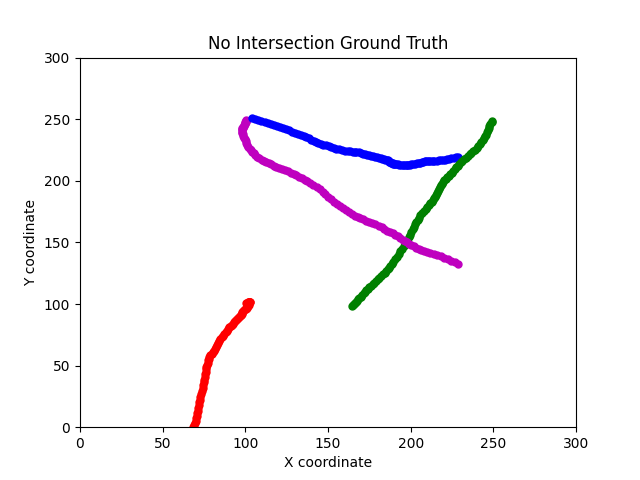
\includegraphics[width=\linewidth,height=0.32\textheight,keepaspectratio]{ground_truth/No Intersection_track.png}\\
      \scriptsize Intersection No Cardinality Change\\
      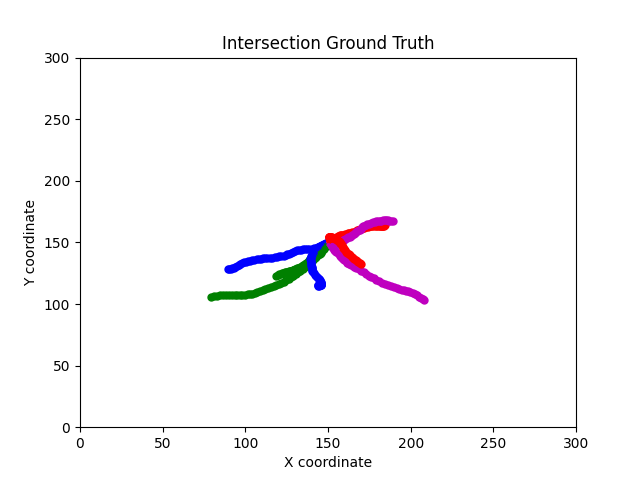
\includegraphics[width=\linewidth,height=0.32\textheight,keepaspectratio]{ground_truth/Intersection_track.png}\\
  \end{column}
  \begin{column}{0.333\linewidth}
      \centering
      \scriptsize No Intersection with Cardinality Change\\
      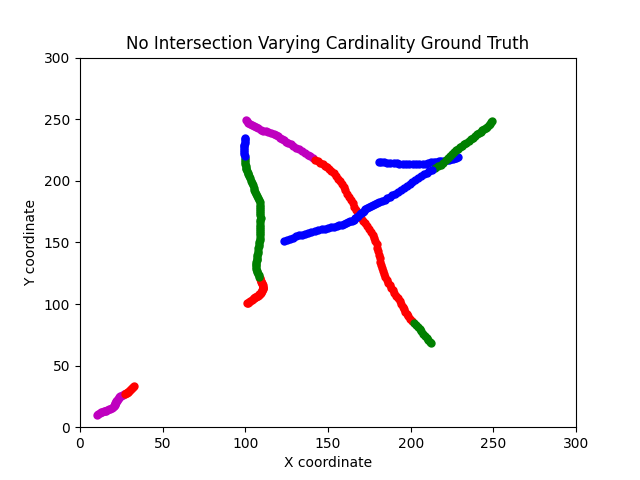
\includegraphics[width=\linewidth,height=0.32\textheight,keepaspectratio]{ground_truth/No Intersection Varying Cardinality_track.png}
      \scriptsize Intersection with Cardinality Change\\
      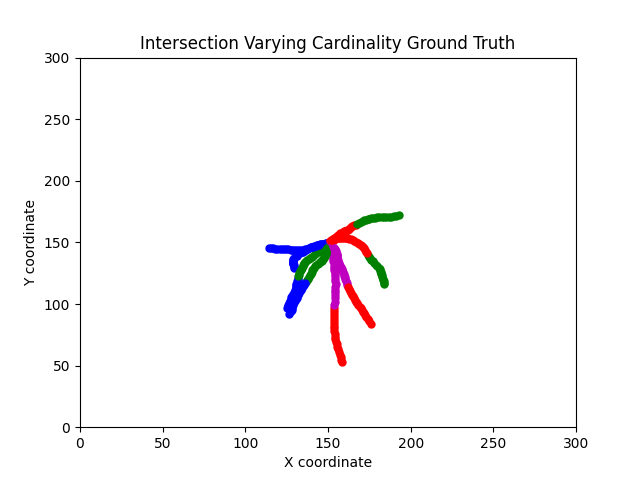
\includegraphics[width=\linewidth,height=0.32\textheight,keepaspectratio]{ground_truth/Intersection Varying Cardinality_track.png}
  \end{column}
  \begin{column}{0.333\linewidth}
      \centering
      \scriptsize Travel in Proximity\\
      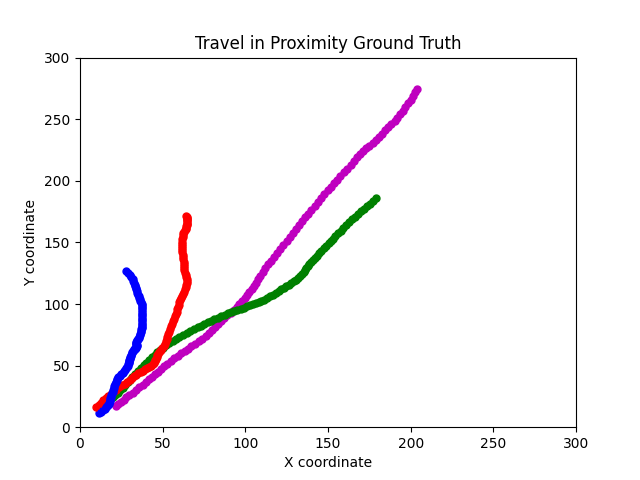
\includegraphics[width=\linewidth,height=0.32\textheight,keepaspectratio]{ground_truth/Travel in Proximity_track.png}\\
      \scriptsize Intersection, Multi-Cardinality Changes\\
      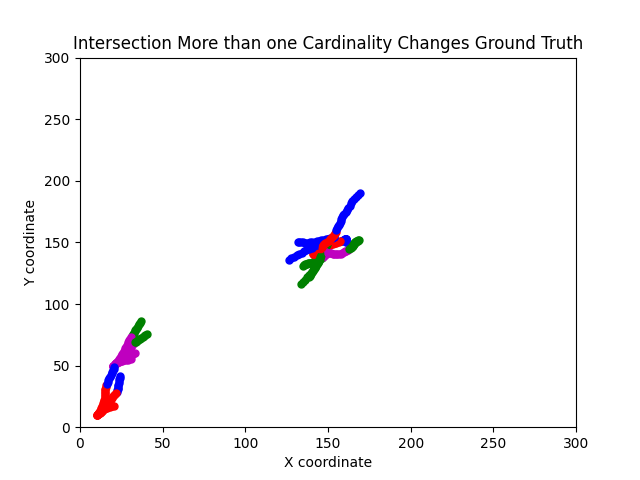
\includegraphics[width=\linewidth,height=0.32\textheight,keepaspectratio]{ground_truth/Intersection More than one Cardinality Changes_track.png}
  \end{column}
\end{columns}
\end{frame}


\begin{frame}{Comparison by using Simulation Data}
\textbf{Scenario 1: No Intersection, No Cardinality Change}
	\begin{itemize}
		    \item In this scenario, four targets are initiated and there would be no intersection whatsoever when the track progresses, also there will be no Cardinality change. 
		    \item The objective of this scenario is to act as a baseline. 
		    \item All trackers should perform relatively well for this scenario.
	\end{itemize}
\end{frame}

\begin{frame}{Comparison by using Simulation Data}
\textbf{Scenario 1: No Intersection, No Cardinality Change}
\begin{columns}[t]
  \begin{column}{0.5\linewidth}
      \centering
      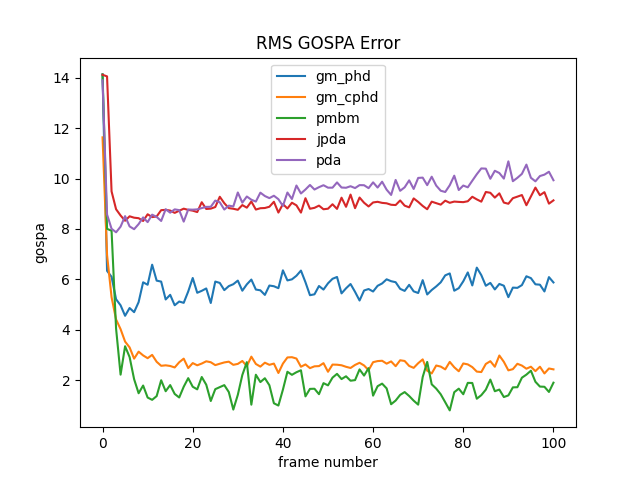
\includegraphics[width=\linewidth,height=\textheight,keepaspectratio]{real_data/scenario1/gospa.png}\\
  \end{column}
    \begin{column}{0.5\linewidth}
      \centering
      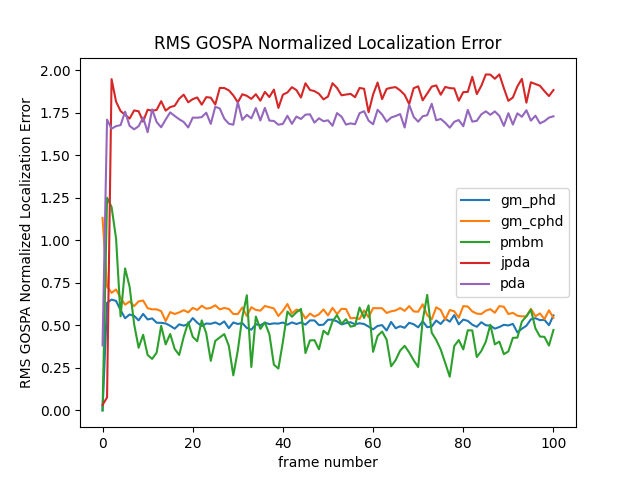
\includegraphics[width=\linewidth,height=\textheight,keepaspectratio]{real_data/scenario1/gospa_localization.png}\\
  \end{column}
\end{columns}
\end{frame}

\begin{frame}{Comparison by using Simulation Data}
\textbf{Scenario 1: No Intersection, No Cardinality Change}
\begin{columns}[t]
  \begin{column}{0.5\linewidth}
      \centering
      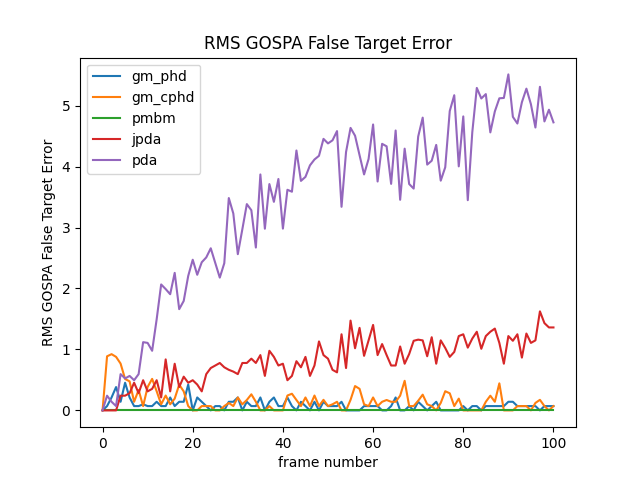
\includegraphics[width=\linewidth,height=\textheight,keepaspectratio]{real_data/scenario1/gospa_false.png}\\
  \end{column}
    \begin{column}{0.5\linewidth}
      \centering
      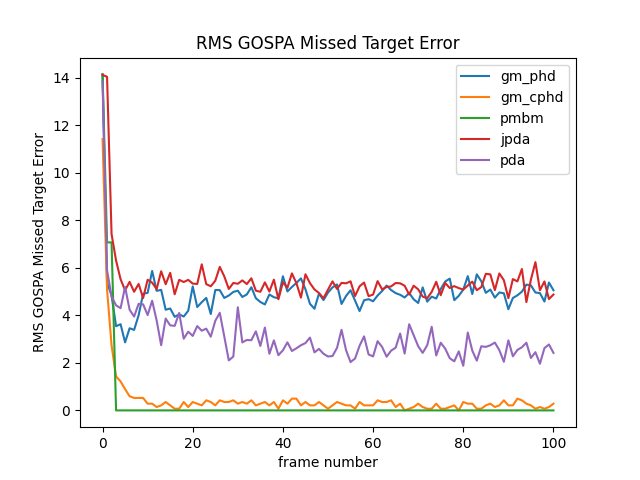
\includegraphics[width=\linewidth,height=\textheight,keepaspectratio]{real_data/scenario1/missed.png}\\
  \end{column}
\end{columns}
\end{frame}


\begin{frame}{Comparison by using Simulation Data}
\textbf{Scenario 2: Intersection, No Cardinality Change}
	\begin{itemize}
		    \item The four tracks will meet at n\_scan/2 steps, and the Cardinality will remain the same through out the simulation. 
		    \item The objective of this scenario is the compare how the 5 trackers fare against the intersection point.
	\end{itemize}
\end{frame}

\begin{frame}{Comparison by using Simulation Data}
\textbf{Scenario 2: Intersection, No Cardinality Change}
\begin{columns}[t]
  \begin{column}{0.5\linewidth}
      \centering
      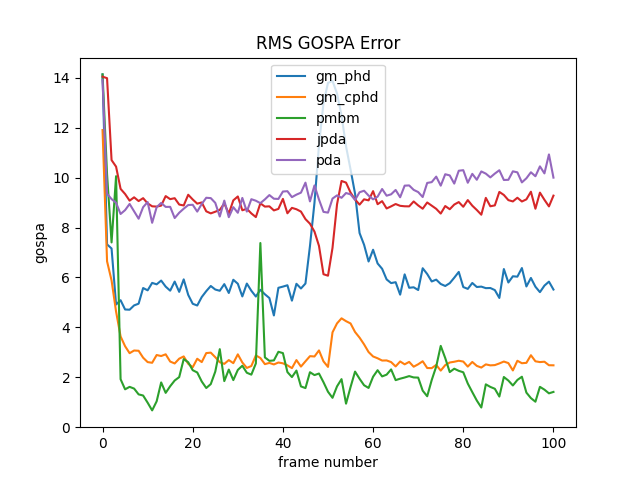
\includegraphics[width=\linewidth,height=\textheight,keepaspectratio]{real_data/scenario2/gospa.png}\\
  \end{column}
    \begin{column}{0.5\linewidth}
      \centering
      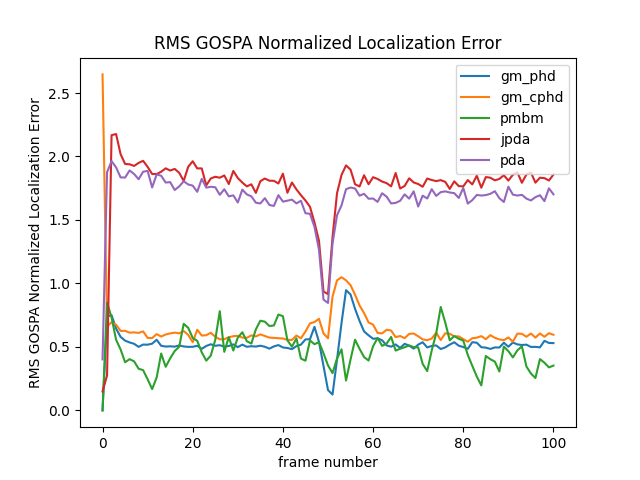
\includegraphics[width=\linewidth,height=\textheight,keepaspectratio]{real_data/scenario2/gospa_localization.png}\\
  \end{column}
\end{columns}
\end{frame}

\begin{frame}{Comparison by using Simulation Data}
\textbf{Scenario 2: Intersection, No Cardinality Change}
\begin{columns}[t]
  \begin{column}{0.5\linewidth}
      \centering
      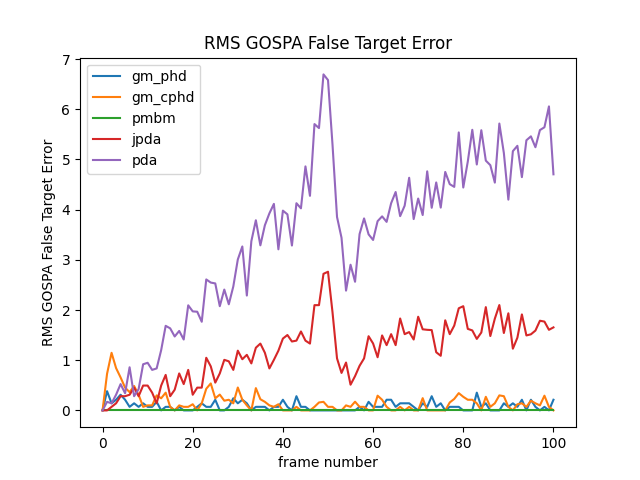
\includegraphics[width=\linewidth,height=\textheight,keepaspectratio]{real_data/scenario2/gospa_false.png}\\
  \end{column}
    \begin{column}{0.5\linewidth}
      \centering
      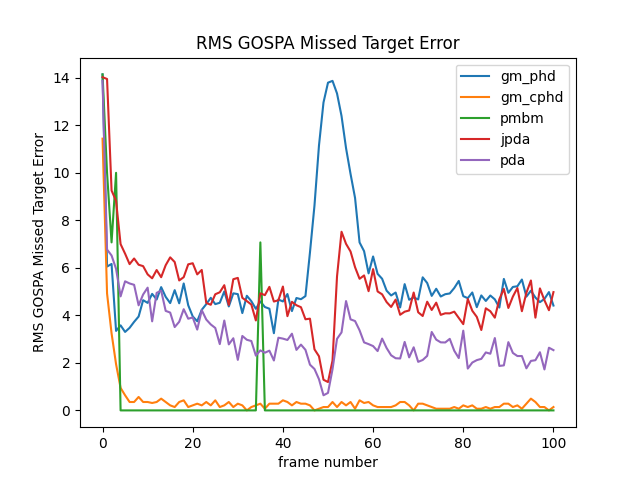
\includegraphics[width=\linewidth,height=\textheight,keepaspectratio]{real_data/scenario2/missed.png}\\
  \end{column}
\end{columns}
\end{frame}


\begin{frame}{Comparison by using Simulation Data}
\textbf{Scenario 3: No Intersection, with Cardinality Change}
	\begin{itemize}
		    \item In this scenario, four targets are initiated and there would be no intersection whatsoever when the track progresses. However, there will be Cardinality changes every 30 scans, in dicated by the color changes in the following graph. 
		    \item The objective of this scenario is to see how the trackers fare against Cardinality variation.
	\end{itemize}
\end{frame}

\begin{frame}{Comparison by using Simulation Data}
\textbf{Scenario 3: No Intersection, with Cardinality Change}
\begin{columns}[t]
  \begin{column}{0.5\linewidth}
      \centering
      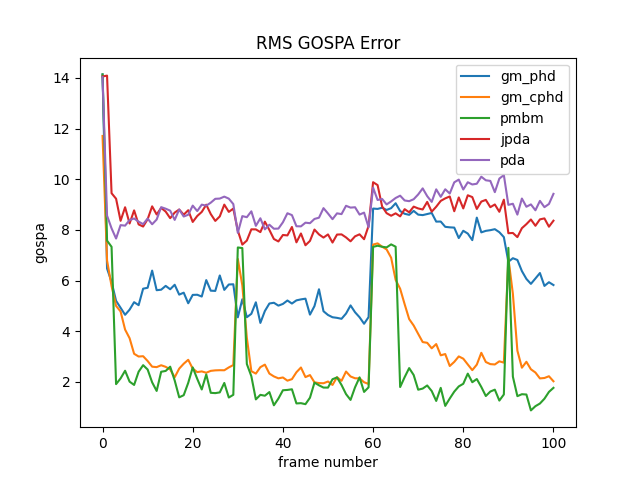
\includegraphics[width=\linewidth,height=\textheight,keepaspectratio]{real_data/scenario3/gospa.png}\\
  \end{column}
    \begin{column}{0.5\linewidth}
      \centering
      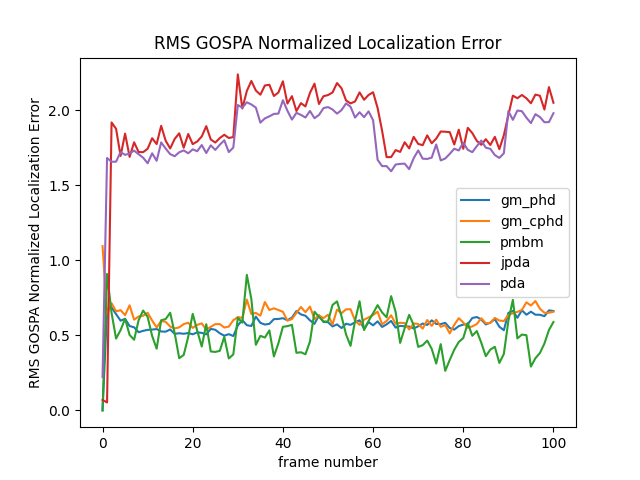
\includegraphics[width=\linewidth,height=\textheight,keepaspectratio]{real_data/scenario3/gospa_localization.png}\\
  \end{column}
\end{columns}
\end{frame}

\begin{frame}{Comparison by using Simulation Data}
\textbf{Scenario 3: No Intersection, with Cardinality Change}
\begin{columns}[t]
  \begin{column}{0.5\linewidth}
      \centering
      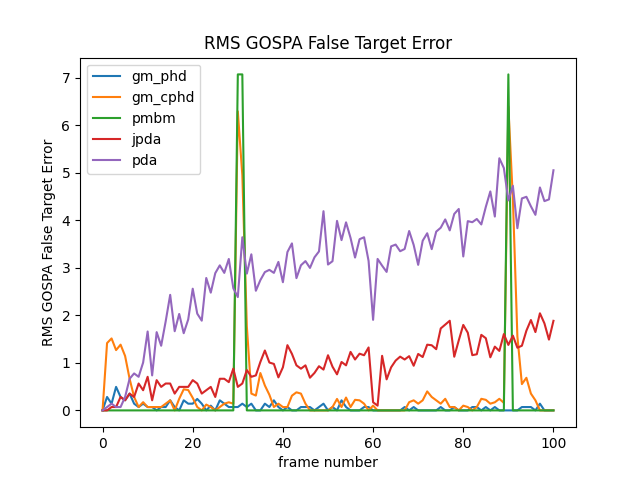
\includegraphics[width=\linewidth,height=\textheight,keepaspectratio]{real_data/scenario3/gospa_false.png}\\
  \end{column}
    \begin{column}{0.5\linewidth}
      \centering
      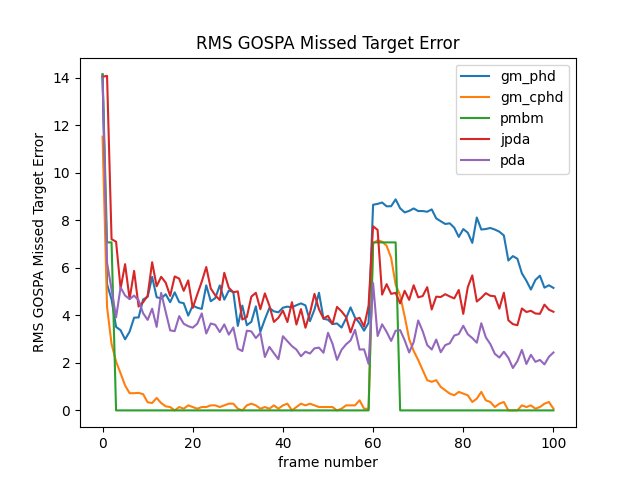
\includegraphics[width=\linewidth,height=\textheight,keepaspectratio]{real_data/scenario3/missed.png}\\
  \end{column}
\end{columns}
\end{frame}


\begin{frame}{Comparison by using Simulation Data}
\textbf{Scenario 4: Intersection, with Cardinality Change}
	\begin{itemize}
		    \item The tracks will meet at n\_scan/2 steps, and the Cardinality will change every 30 scans. 
		    \item The objective of this scenario is the compare how the 5 trackers fare against the intersection point and Cardinality variation. 
	\end{itemize}
\end{frame}

\begin{frame}{Comparison by using Simulation Data}
\textbf{Scenario 4: Intersection, with Cardinality Change}
\begin{columns}[t]
  \begin{column}{0.5\linewidth}
      \centering
      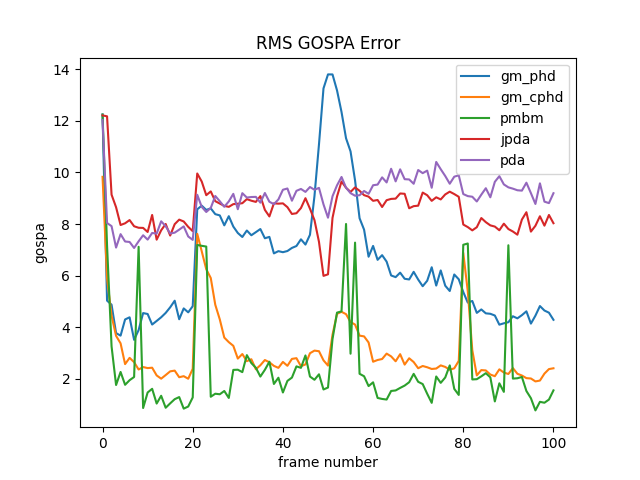
\includegraphics[width=\linewidth,height=\textheight,keepaspectratio]{real_data/scenario4/gospa.png}\\
  \end{column}
    \begin{column}{0.5\linewidth}
      \centering
      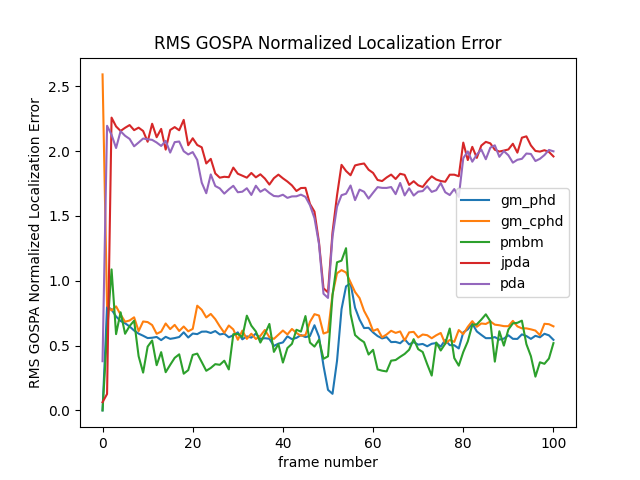
\includegraphics[width=\linewidth,height=\textheight,keepaspectratio]{real_data/scenario4/gospa_localization.png}\\
  \end{column}
\end{columns}
\end{frame}

\begin{frame}{Comparison by using Simulation Data}
\textbf{Scenario 4: Intersection, with Cardinality Change}
\begin{columns}[t]
  \begin{column}{0.5\linewidth}
      \centering
      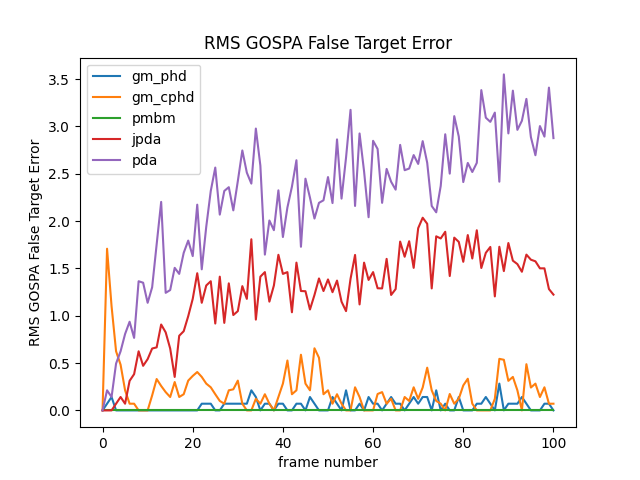
\includegraphics[width=\linewidth,height=\textheight,keepaspectratio]{real_data/scenario5/gospa_false.png}\\
  \end{column}
    \begin{column}{0.5\linewidth}
      \centering
      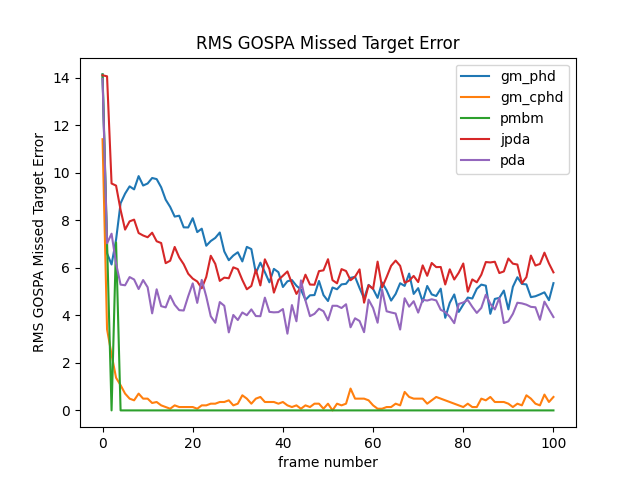
\includegraphics[width=\linewidth,height=\textheight,keepaspectratio]{real_data/scenario5/missed.png}\\
  \end{column}
\end{columns}
\end{frame}


\begin{frame}{Comparison by using Simulation Data}
\textbf{Scenario 5: Travel in Proximity}
	\begin{itemize}
		    \item This scenario has 4 targets travel in proximity, without any Cardinality changes.
		    \item This scenario is designed to mimic the road traffic where cars are moving in parallel with each other closely.
	\end{itemize}
\end{frame}

\begin{frame}{Comparison by using Simulation Data}
\textbf{Scenario 5: Travel in Proximity}
\begin{columns}[t]
  \begin{column}{0.5\linewidth}
      \centering
      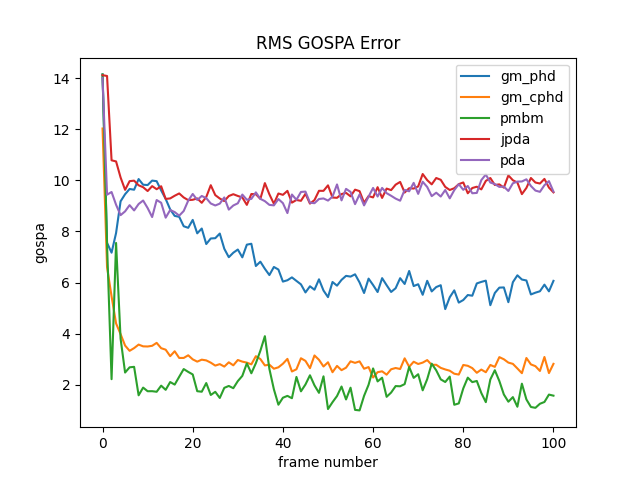
\includegraphics[width=\linewidth,height=\textheight,keepaspectratio]{real_data/scenario5/gospa.png}\\
  \end{column}
    \begin{column}{0.5\linewidth}
      \centering
      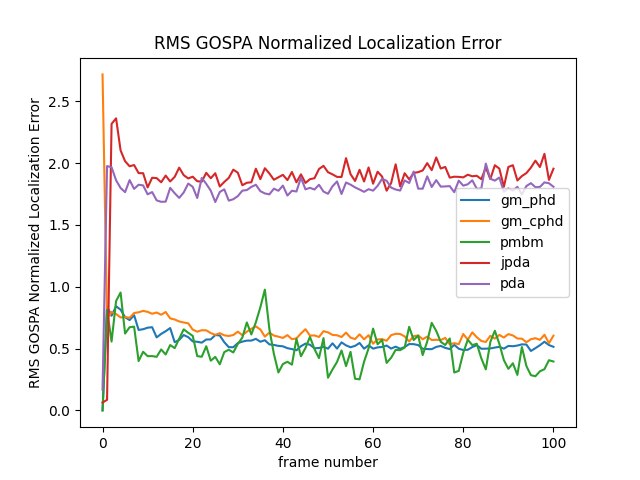
\includegraphics[width=\linewidth,height=\textheight,keepaspectratio]{real_data/scenario5/gospa_localization.png}\\
  \end{column}
\end{columns}
\end{frame}

\begin{frame}{Comparison by using Simulation Data}
\textbf{Scenario 5: Travel in Proximity}
\begin{columns}[t]
  \begin{column}{0.5\linewidth}
      \centering
      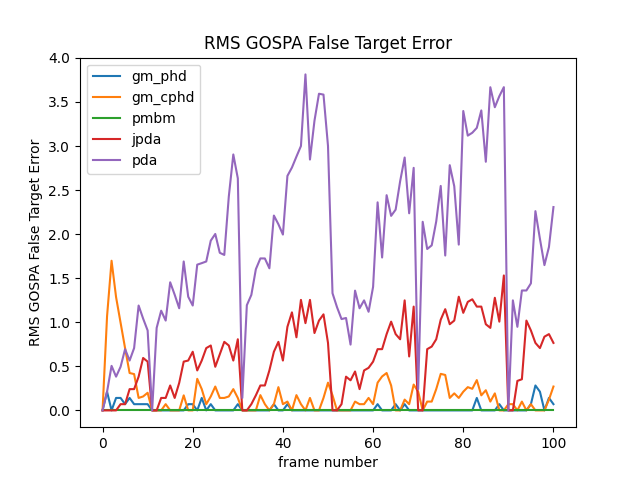
\includegraphics[width=\linewidth,height=\textheight,keepaspectratio]{real_data/scenario6/gospa_false.png}\\
  \end{column}
    \begin{column}{0.5\linewidth}
      \centering
      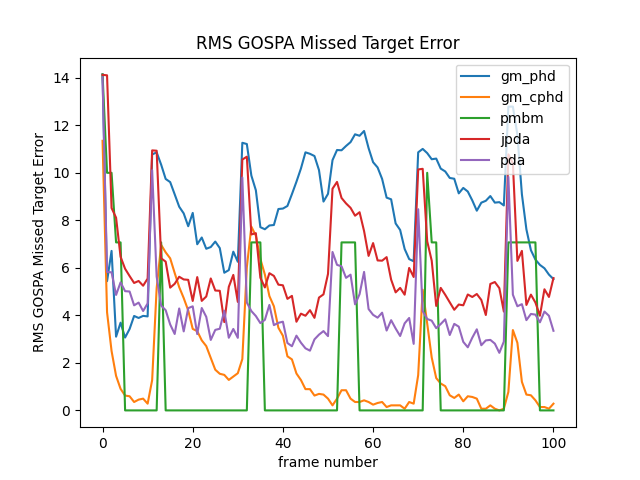
\includegraphics[width=\linewidth,height=\textheight,keepaspectratio]{real_data/scenario6/missed.png}\\
  \end{column}
\end{columns}
\end{frame}


\begin{frame}{Comparison by using Simulation Data}
\textbf{Scenario 6: Intersection, with Multiple Cardinality Change}
	\begin{itemize}
		    \item This scenario is designed to be the highest difficulty. At n\_scan/2 step, there would be intersection. There would also be multiple varying Cardinalities, such as disappearing of more than one object and appearing of more than one object simultaneously.
	\end{itemize}
\end{frame}

\begin{frame}{Comparison by using Simulation Data}
\textbf{Scenario 6: Intersection, with Multiple Cardinality Change}
\begin{columns}[t]
  \begin{column}{0.5\linewidth}
      \centering
      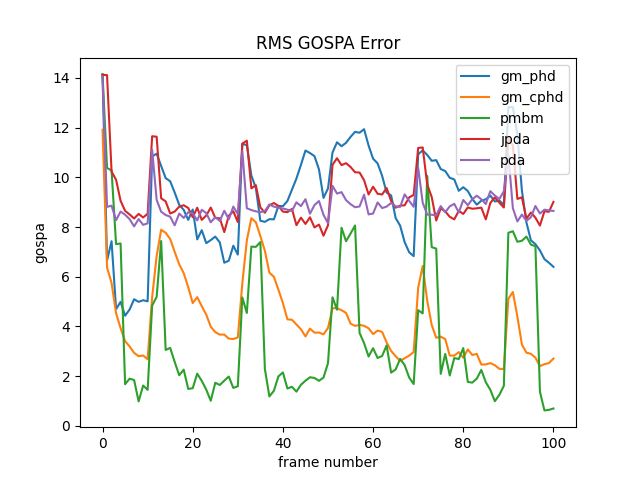
\includegraphics[width=\linewidth,height=\textheight,keepaspectratio]{real_data/scenario6/gospa.png}\\
  \end{column}
    \begin{column}{0.5\linewidth}
      \centering
      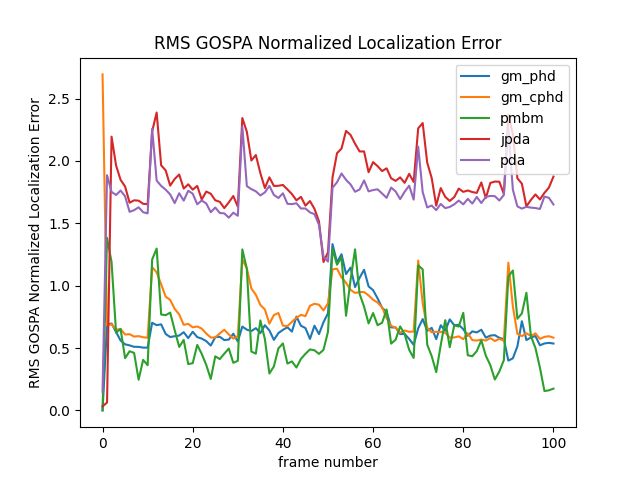
\includegraphics[width=\linewidth,height=\textheight,keepaspectratio]{real_data/scenario6/gospa_localization.png}\\
  \end{column}
\end{columns}
\end{frame}

\begin{frame}{Comparison by using Simulation Data}
\textbf{Scenario 6: Intersection, with Multiple Cardinality Change}
\begin{columns}[t]
  \begin{column}{0.5\linewidth}
      \centering
      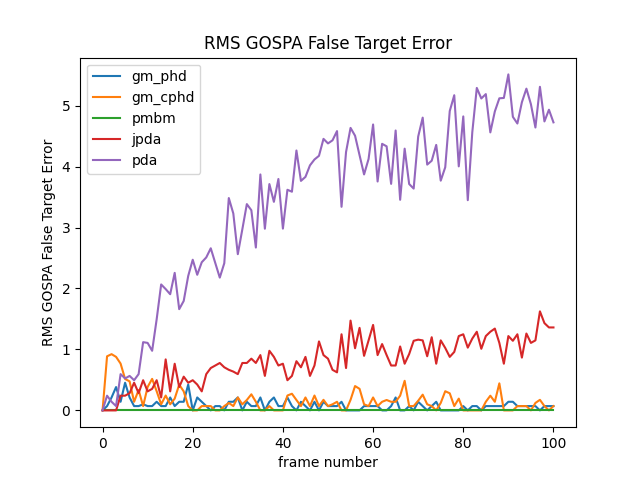
\includegraphics[width=\linewidth,height=\textheight,keepaspectratio]{real_data/scenario1/gospa_false.png}\\
  \end{column}
    \begin{column}{0.5\linewidth}
      \centering
      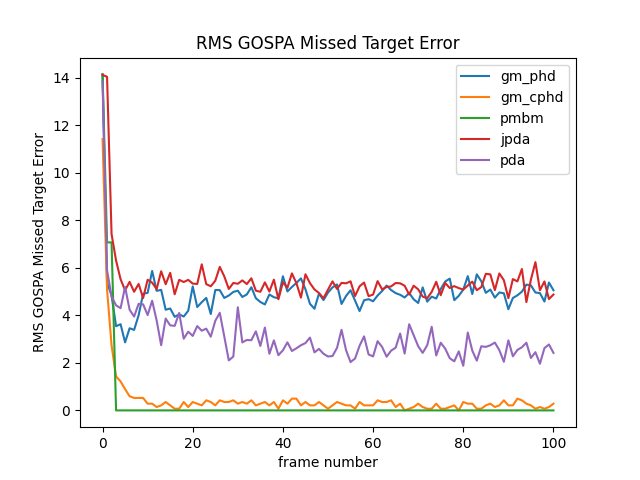
\includegraphics[width=\linewidth,height=\textheight,keepaspectratio]{real_data/scenario1/missed.png}\\
  \end{column}
\end{columns}
\end{frame}

\begin{frame}{Project Overview}
\textbf{NuScenes Data: N Different Scenarios}

\end{frame}

\begin{frame}{Comparison by using NuScenes Data}

\end{frame}

\begin{frame}{Comparison by using NuScenes Data}

\end{frame}

\begin{frame}{Comparison by using NuScenes Data}

\end{frame}

\begin{frame}{Comparison by using NuScenes Data}

\end{frame}


\end{document}